\documentclass{mprop}
\usepackage{graphicx}
\usepackage{hyperref}
\usepackage{url}
\usepackage{amsmath}
% alternative font if you prefer
%\usepackage{times}

% for alternative page numbering use the following package
% and see documentation for commands
%\usepackage{fancyheadings}


% other potentially useful packages
\usepackage{epigraph}
%\uspackage{amssymb,amsmath}
%\usepackage{fancyvrb}
%\usepackage[final]{pdfpages}

% Inspirational Quote type setting
\makeatletter
\newenvironment{chapquote}[2][2em]
  {\setlength{\@tempdima}{#1}%
   \def\chapquote@author{#2}%
   \parshape 1 \@tempdima \dimexpr\textwidth-2\@tempdima\relax%
   \itshape}
  {\par\normalfont\hfill--\ \chapquote@author\hspace*{\@tempdima}\par\bigskip}
\makeatother

\begin{document}

%%%%%%%%%%%%%%%%%%%%%%%%%%%%%%%%%%%%%%%%%%%%%%%%%%%%%%%%%%%%%%%%%%%
\title{Securing and Integrating the IoT with a Smart Home Router}
\author{Fergus W. Leahy}
\date{16/12/2013}
\maketitle
%%%%%%%%%%%%%%%%%%%%%%%%%%%%%%%%%%%%%%%%%%%%%%%%%%%%%%%%%%%%%%%%%%%

%%%%%%%%%%%%%%%%%%%%%%%%%%%%%%%%%%%%%%%%%%%%%%%%%%%%%%%%%%%%%%%%%%%
\tableofcontents
\newpage
%%%%%%%%%%%%%%%%%%%%%%%%%%%%%%%%%%%%%%%%%%%%%%%%%%%%%%%%%%%%%%%%%%%

%%%%%%%%%%%%%%%%%%%%%%%%%%%%%%%%%%%%%%%%%%%%%%%%%%%%%%%%%%%%%%%%%%%
\section{Introduction}
\label{sec:introduction}

\begin{chapquote}{Mark Weiser, \textit{The Computer for the Twenty-First Century, 1991}}
    ``The most profound technologies are those that disappear. They weave themselves into the fabric of everyday life until they are indistinguishable from it.''
\end{chapquote}

The modern home is becoming increasingly filled with a variety of \textit{connected} devices (laptops, tablets, phones, set-top boxes etc.), providing a myriad of different services to users within the home. On top of this, with the advent use of smart phones and introduction of wearable devices, we too are starting to carry around our own personal network of devices everywhere we go, brushing past many others in our daily lives at home, work and on the street. Although all connected to the Internet, these devices are often encapsulated within their own environment and ecosystem, unable to interconnect, creating a fractured and often complex user experience. 

Making matters more interesting, the Internet of Things paradigm is once again becoming a field of great interest due to the advent of cheap, low power wireless embedded devices \cite{2013IoT}. However, not much consideration has been made for how these Things should be integrated into the existing home network, with many approaches opting to simply bridge the device to the cloud (\cite{SmartThings}, \cite{Twine}, \cite{IETF_CORE}), with obvious concerns for security, privacy and up-time.

As these devices enter our homes and pockets, bringing with them their own ecosystems, the user is faced with the increasingly difficult burden of managing all of them and the ecosystems \cite{brundell2011w}, \cite{brown2013multinet}. Due to the sheer number and diversity of these devices, many of which will provide overlapping services and functionality, problems arise in how to ensure these devices not only play nicely together but also ensuring the user's network and information stays secure against new and unanticipated threats.

In order for these multiple layered networks of devices to truly fade away into the fabric of our everyday lives, a platform and relevant protocols need to be engineered to not only support this heterogeneous network securely, but also aid the user in managing both the network and the privacy of their information.

The Homework home router platform was created to these issues. Rather than assume every user is a network administrator, the project investigated the needs and abilities of the average user in order to propose the future of home networking, re-inventing the protocols, models and architectures to truly suit the home environment. This re-invention of the home router allows a user to easily install, manage and use their home network, without the need of a Cisco qualification.

In regards to the Internet of Things development, previous work demonstrated that it was in need a suitable protocol in order to meet the specific needs of a network of Things \cite{KNoT}. Thus, a new protocol was designed and implemented, which could not only run on even the most constrained battery-powered devices (8MHz), but it could also efficiently scale to support hundreds of Things within the same network.

%TODO: WRITE MORE LINKY LINKY

%briefly explain the context of the project problem

%%%%%%%%%%%%%%%%%%%%%%%%%%%%%%%%%%%%%%%%%%%%%%%%%%%%%%%%%%%%%%%%%%%

\section{Statement of Problem}

The Internet of Things protocol created in \cite{KNoT} proved to be a successful proof-of-concept; However, in order for it to be considered for deployment and integration into existing homes, several issues need to first be addressed.

\begin{itemize}
    \item [Security:] Due to time constraints the initial design of the IoT protocol didn't consider security concerns. However, the IoT protocol needs to be sufficiently secured to prevent eavesdropping of the transmitted data and injection of false events by perpetrators masquerading as sanctioned participants in the network. 
    \item [Integration:] The current implementation exists as a standalone component with several demo applications. Integration of the IoT protocol into a user-friendly platform is necessary to harness the full power of the Thing's network. The integrated platform would then be able to search and connect to available Things, receive events from the sensors and using user customised rules, use automata to detect if the received events match and then perform actions by pushing commands to actuators in the network.
\end{itemize}

\subsection{Intranet of Things vs Internet of Things} % (fold)
\label{sub:intranet_of_things}

As described earlier in section \ref{sec:introduction}, many previous deployments of Internet of Things networks have taken a cloud first approach, see \cite{SmartThings, Twine}. Whilst this yields certain benefits, such as easy external access and integration with other services \cite{IFTTT, Xively}, it also poses several questions regards data security, privacy and up-time. For this project, the focus will be on developing a home first platform, in which all Things communication will be kept local, with no cloud processing involved; Thus a more suitable name, the Intranet of Things, will be used. 
% subsection intranet_of_things (end)


\subsection{Project Outcomes} % (fold)
\label{sub:project_outcomes}

Outcomes of the project:
\begin{itemize}
  \item[-] An extended IoT protocol with sufficient security to prevent eavesdropping and unsanctioned devices.
  \item[-] An Extended home information platform (Homework), with the IoT controller role implemented, enabling capturing of IoT events from sensors and creation of commands for actuators.
  \item[-] Use of Homework's automata to implement closed loop control of Things in the home, subscribing to sensor events, processing rules and publishing to actuators to perform actions.
\end{itemize}
% subsection subsection_name (end)

% clearly state the problem to be addressed in your forthcoming project. Explain why it would be worthwhile to solve this problem.

%%%%%%%%%%%%%%%%%%%%%%%%%%%%%%%%%%%%%%%%%%%%%%%%%%%%%%%%%%%%%%%%%%%
\section{Literature Review}
This section discusses previous work on Internet of Things protocols, WSN security and home networking which provides the motivation and possible aid in solving the previously mentioned issues.

\subsection{State-of-the-art IoT Protocols} % (fold)
\label{sub:state_of_the_art_iot_protocols}
Over the last 20 years, the Internet of Things has developed and evolved continuously, from 20 years ago where it was the concept of using barcodes, and later RFID\cite{K.Ashton}, to track items in a warehouse, to today where our home appliances are filled with ``smart'' electronics, able to sense, react and notify the user of events, such as the washing machine finishing a load. Whilst the Internet of Things has been around for quite some time, under various guises, it's yet to become commercially successful and see wide-spread deployment; Many believe that 2013 is the year that the Internet of Things will truly take off and become ubiquitous in our daily lives\cite{2013IoT}.

The rest of this section will discuss the various different attempts made to create Internet of Things networks in the home.

\subsubsection{Smart Things} % (fold)
\label{ssub:smart_things}
Launched in 2012, the SmartThings platform aims to allow the user to turn any ordinary object in the home into a ``Smart'' object by giving it the ability to connect to the Internet. The platform consists of a central hub connected to the Internet, containing a low-power Zigbee radio, from which it connects to an array of SmartThings accessories as well as many pre-existing third party Zigbee devices. Some of these accessories include motion detectors, moisture sensors, vibration detectors, power-plug switches as well as many others. The user can then view and interact with their Smart Things through the cloud service via an Internet-connected PC or a smartphone, allowing them to either control the devices directly or set-up rules/schedules for devices.

\begin{figure}[h!]
\centering
    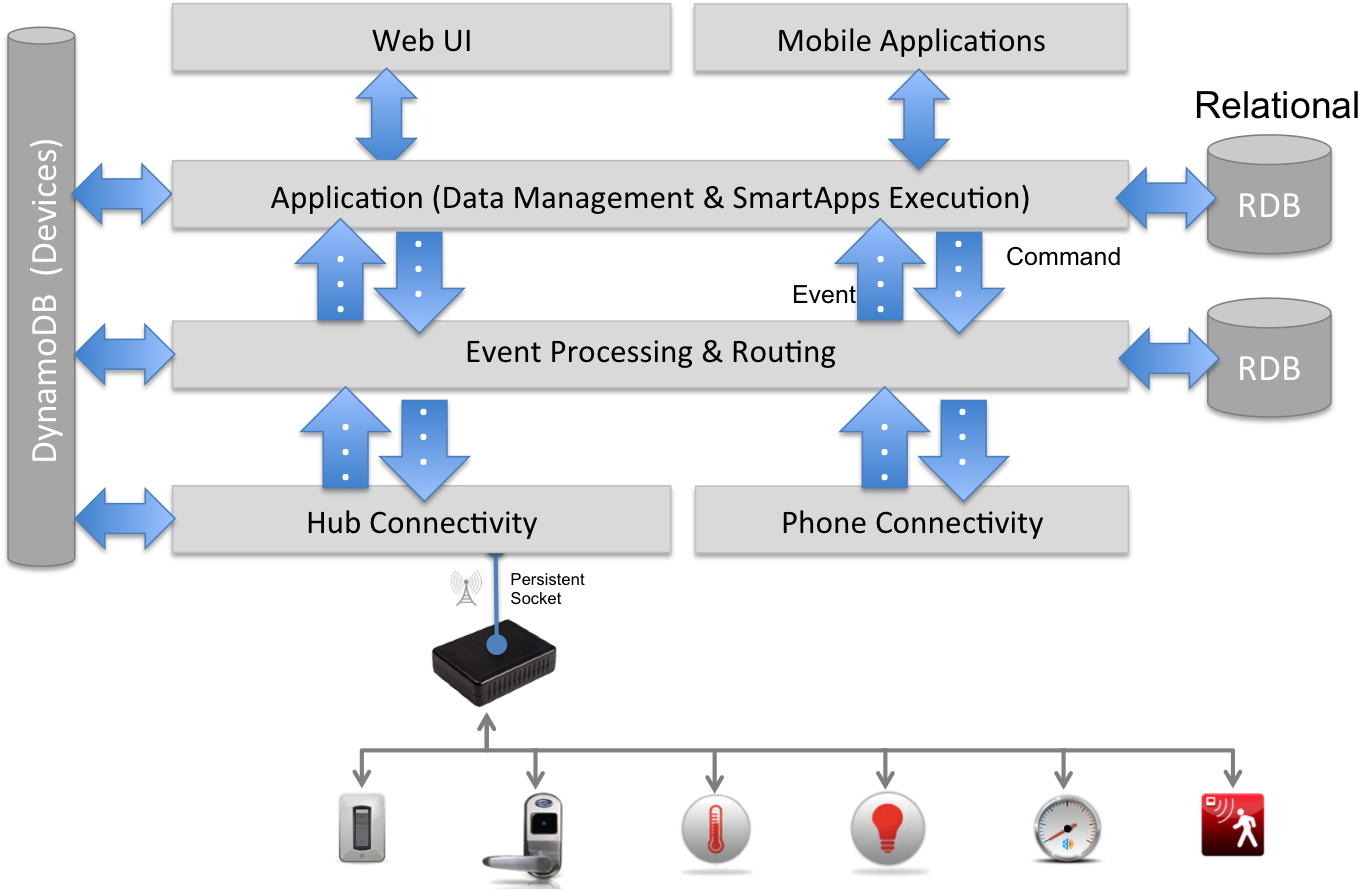
\includegraphics[scale=0.4]{images/smartThingsCloudFirstDiagram.png}
    \caption[]{Smart Things - Cloud approach\footnotemark}
    \label{fig:cloud}
\end{figure}
\footnotetext{Image from Smart Things developer support: \url{https://support.smartthings.com/entries/21603009-Device-Types-Capabilities-Attributes}}

As shown in figure \ref{fig:cloud}, Smart Things takes a cloud approach, offloading all processing to the cloud, leaving the hub to just act as a gateway and translator between the Things and the cloud. By utilising the cloud in this way, it enables the hub to be a very simple and low-power device, reducing both the purchasing and running costs for the user. It also allows the user to access their network of Things from anywhere, at any time, which would otherwise be difficult to do in a local approach. 

However, the cloud approach also has several drawbacks. By offloading the entire processing needs of the network, as show above, the network of Things becomes vulnerable to failure if either the network fails or is unresponsive, or if the cloud service fails or goes down for maintenance. Another issue is the privacy of the user's data; How safe is the data in the cloud and how secure are the services they make available for users to interact with their devices with. There have been many examples of online services that have been attacked, leaking user data and/or shutting down for extended periods of time \cite{Playstation, Amazon, Google}.

Talk about integration of two home networks.


% Currently, there is no information on how the underlying protocol for connecting the SmartThings to the hub works, but at the time of writing, the current implementation uses a ``cloud first'' approach. This means that rather than the hub wiring all devices together based on the rules and schedules set up by the user, all the intelligence of the network is being handled in the cloud. This brings about the problem of Internet connectivity, with two points of failure, either the user or the cloud. From the user's standpoint, an Internet connection might not be available where the hub is located, or the user could have a faulty, slow or non-permanent connection, which renders all the SmartThings devices into dumb devices. In contrast to this, because of the reliance on the cloud, if the cloud service provider experiences downtime then all SmartThings users devices become dumb devices. In cases where these devices are used for security and safety, dire consequences could result.
% subsubsection smart_things (end)

\subsubsection{CoRE CoAP HIP-DEX} % (fold)
\label{ssub:core_coap}

% subsubsection core_coap (end)
\subsubsection{KNoT} % (fold)
\label{ssub:knot}

% subsubsection knot (end)
% subsection state_of_the_art_iot_protocols (end)

\subsection{Homework - Smart Home Router} % (fold)
\label{sub:homework_smart_home_router}
\textbf{Discuss Homework router and cache db}
% subsection homework_smart_home_router (end)

%%%%%%%%%
\subsection{Symmetric Security - TinySec, MiniSec, ContikiSec} % (fold)
\label{sub:tinysec_minisec_contikisec}

\subsubsection{TinySec} % (fold)
\label{ssub:tinysec}
TinySec is a fully functional symmetric security link layer component created for the wireless sensor network operating system, TinyOS. It was the first fully implemented solution for WSNs and was created to address the security worries of running a WSN and transmitting private sensor data in the clear. Unlike conventional security protocol implementations which can afford significant time and space overheads, such as 16-32 bytes for security per packet, WSN typically run on extremely constrained devices with packet sizes of just 30 bytes, making those implementations impossible/extremely expensive to run.

To resolve this, TinySec took a balanced approach making a compromise between the level of security, packet overhead and resource requirements. The end result proved that it's possible to secure a WSN efficiently entirely in software, without the need for additional hardware. 

Communication between nodes, not just nodes-to-base-station, in WSNs is often quite important, allowing nodes to not only redirect other's traffic along routes but also consolidate duplicate packets from multiple nodes about the same event, saving the overall network from wasting power receiving and transmitting the extra packets; tinySec chose to engineer in security at the link layer, allowing these mechanisms to perform without alteration. The security goals of TinySec aimed to enable access control, whereby only authorised participants may participate in the network, with unauthorised messages easy to spot and reject; ensure message integrity, so that authorised messages can't be illegally altered by a man-in-the-middle without the receiver noticing; and ensure confidentiality, to ensure information is kept secret from unauthorised eavesdroppers. 

The TinySec implementation uses Cipher Block Chaining with an initialisation vector (IV), together these achieve semantic security, therefore ensuring that encrypting the same plain text twice returns a different cipher text each time. So that the receiving end knows how to begin decryption of the data, the IV must be sent in the clear along with the encrypted data. When using an IV, its length needs to be taken into consideration because repeats will occur when the number wraps, causing a security vulnerability. On unconstrained devices an IV is usually 8 or 16 bytes, however due to the packet size limitations of the wireless sensors used, a 8(2 byte counter) byte IV was chosen. In the IV, 6 bytes are made up of pre-existing fields to conserve space and ensure globally unique IVs in the network e.g. to nodes send the same data event and both happen to have the same counter value, but differ in source (src), so the IV is different, therefore preserving the security.

For ensuring authenticity and integrity of messages, TinySec uses Cipher Block Chaining Message Authentication Codes (CBC-MAC) of 4 bytes in length. Similar to a CRC, CBC-MAC runs over the data and produces a 4 byte MAC which is appended to the packet. If a message was to be altered, the attacker has a 1 in $2^{32}$ of blindly forging a valid MAC. In a WSN with a limited send rate of 19.2Kb/s it would take over 20 months to send enough packets to possibly succeed in forging a MAC. In the case of attack, a receive heuristic could be used to detect multiple failed MAC transmissions at a nearby node, triggering an alert to the rest of the network.

Whilst TinySec can secure a WSN against eavesdropping and forged messages, it has two significant drawbacks. Firstly, in regards to key distribution, encryption and authentication keys need to be loaded to the nodes prior to deployment. This can cause issues when the shared keys need to be changed, such as when they are compromised, as all nodes in the network will need the new key. This can be especially difficult post-deployment, simply due to the number of nodes and often embedded and/or difficult to reach locations. Secondly, if a node in the network is compromised, because the authentication key is a network wide shared key, the illegitimate node can pretend to be any other node in the network, making it difficult to protect, never mind counter against.
% subsubsection tinysec (end)

\subsubsection{MiniSec} % (fold)
\label{ssub:minisec}
MiniSec was created to tackle several problems apparent in the then current WSN security protocols, TinySec and Zigbee \cite{MiniSec}. The pre-cursor to MiniSec, TinySec, received much attention and use due to its power and resource efficient security implementation, but because of limited authentication and lack of replay prevention, the overall security provided was deemed insufficient to protect a WSN. A commercial alternative, Zigbee, exhibits significantly higher security, but does so at the cost of higher energy consumption. MiniSec was designed to find the middle-ground between the two, increasing security whilst remaining energy efficient. 

In contrast to TinySec, for its encryption mode of operation, MiniSec uses Offset Code Book. Unlike cipher block chaining (CBC) which requires two passes to provide both encryption and authentication, OCB provides both in only one pass over the data. This one pass also performs faster that CBC's two passes and only requires one key for operation, thus making it more appropriate for a constrained device in terms of power and storage. 

MiniSec also differs from TinySec by reducing the size of the IV counter sent in a packet, yet managing to increase the size of the IV so that it wraps less often. This is achieved by storing some state about the IV counter locally and only transmitting the last n bits of it to the receiving node. This also requires some logic on both sides to manage the counter in the event of packet loss larger than the range of values stored in the last n bits sent, i.e. when $>2^n$ are lost. For MiniSec, the authors chose n = 3. Because of this, only 3 extra bits needed to be sent with a packet, instead of the 2 extra bytes in TinySec. However, this overhead could be removed altogether. The maximum default packet size in TinyOS is 29 bytes, therefore the 3 most significant bits in the packet-size byte aren't used and can instead be used to store the IV counter. Therefore the need for the extra byte to store those bits is eliminated.\footnote{The publicly available source code for MiniSec (\url{https://sparrow.ece.cmu.edu/group/minisec.html}) does not make use of this technique, instead it appends an additional byte, thus reducing the benefit of the proposed reduced packet-size state-based counter.}

Another improvement, is the use of the synchronised counter (also used as the IV) to prevent replay attacks. As each packet is received, the counter is incremented accordingly, thus if a packet arrives with a counter less than the one stored locally, it is dropped as one can determine it must be a replayed packet. 

% subsubsection minisec (end)

\subsubsection{ContikiSec} % (fold)
\label{ssub:contikisec}
Similar to TinySec\cite{TinySec} and MiniSec\cite{MiniSec}, ContikiSec \cite{ContikiSec} is an asymmetric cryptographic security network layer, however, it's built for the other significant WSN OS, Contiki, instead of TinyOS. The paper presents two main contributions; first, an extensive evaluation of several block-ciphers and modes-of-operation, comparing ROM/RAM sizes and timings; second, a modular asymmetric encryption network layer for Contiki, offering modes for encryption, authentication or encryption + authentication.

After comparing several block ciphers (AES, Skipjack, RC5, Triple-DES, Twofish and XTEA), AES was chosen for use in ContikiSec due to its good trade-off between resource consumption and security. This is in contrast to both TinySec and MiniSec, which chose to use Skipjack. At the respective times of publication of TinySec and MiniSec, Skipjack was deemed sufficiently secure by NIST until 2008. Similar to MiniSec, ContikiSec also uses offset codebook as its mode of operation, combining both encryption and authentication into one pass.
% subsubsection contikisec (end)
\cite{TinySec, luk2007minisec, ContikiSec}
% subsection tinysec_minisec_contikisec (end)
%%%%%%%%%

\subsection{Key Distribution Problem} % (fold)
\label{sub:key_distribution_problem}
Tried to solve using Faraday cages...\cite{MessageBottle}
Propose to use Asymmetric Security aka Public Key crypto
% subsection key_distribution_problem (end)

\subsection{Asymmetric Security - TinyECC and Certificates} % (fold)
\label{sub:asymmetric_security}
\subsubsection{TinyECC} % (fold)
\label{ssub:tinyecc}
\cite{TinyECC}
A public key crypto implementation of Elliptic Curve cryptography, supporting higher effective security with smaller keys (than RSA).
As previously discussed, public key cryptography (PKC) using traditional algorithms, such as RSA, has had a limited deployment in WSN due to its high computational cost and implementation size. In cases where it has been used, such as TinyPK, implementations only use a subset of the operations on the sensor node in order to reduce the long temporal overhead associated with them; however, this also reduces the effectiveness of the security and forces workarounds to be created, as TinyPK demonstrated.

As an alternative to RSA and other typical algorithms, elliptic curve cryptography (ECC) shows promise for using PKC on WSNs, due to its lower computational overhead, enabling both public and private operations to be carried out on a sensor node, as well as it reduced key size and compact signatures, not only consuming less storage but also reducing lengthy public key packet transmissions. This is achieved whilst maintaining the equivalent security as RSA\cite{ECC} e.g. a 1024-bit RSA key size is equal in security to a 160-bit ECC key size. These benefits make it far for suitable for use on WSNs when compared to RSA, thus removing the need to offload work to other, more power, devices\cite{TinyPK}.

TinyECC \cite{TinyECC} is an implementation of ECC for the TinyOS WSN OS, featuring a full set of public and private key operations, unlike TinyPK. It also has various optimisation switches, allowing developers to balance implementation size against performance. TinyECC was tested on a variety of TinyOS-compatible constrained sensor platforms, including MICAz, TelosB, Tmote Sky and Imote2, extensively proving that it's feasible for a wide range of WSN platforms.

As mentioned in TinyPK, private key operations for signing blocks of data took in the order of tens of minutes\cite{TinyPK}, whereas, with the use of ECC, TinyECC achieves the same operation in 1.6s when all optimisations are used. Similarly, TinyECC also achieves encryption speeds of 3.3s/pkt and decryption speeds of 2.1s/pkt. Whilst these rates are several orders of magnitude slower than symmetric algorithms, they are only normally used for a short period when securely bootstrapping keys for symmetric cryptography, which would then be used after completion.
% subsubsection tinyecc (end)

\subsubsection{Certificates and Public Key Infrastructures} % (fold)
\label{ssub:certificates_and_public_key_infrastructures}
Discuss the use of certificates and certificate authority to pass trust up the chain.
% subsubsection certificates_and_public_key_infrastructures (end)
% subsection asymmetric_security (end)


\subsection{Other Works} % (fold)
\label{sub:other_works}
\subsubsection{MQTT} % (fold)
\label{ssub:mqtt}

% subsubsection mqtt (end)
\subsubsection{IETF Work} % (fold)
\label{ssub:ietf_work}
\cite{IETF_COAP_HTTP, IETF_CORE}
% subsubsection ietf_work (end)
% subsection other_works (end)

% present an overview of relevant previous work including articles, books, and existing software products. Critically evaluate the strengths and weaknesses of the previous work.

%%%%%%%%%%%%%%%%%%%%%%%%%%%%%%%%%%%%%%%%%%%%%%%%%%%%%%%%%%%%%%%%%%%
\section{Proposed Approach}

% state how you propose to solve the software development problem. Show that your proposed approach is feasible, but identify any risks.
\subsection{Security Architecture} % (fold)
\label{sub:security_architecture}

\subsubsection{Symmetric Key Cryptography} % (fold)
\label{ssub:symmetric_key_cryptography}

% subsubsection symmetric_key_cryptography (end)
\subsubsection{Asymmetric Key Cryptography} % (fold)
\label{ssub:asymmetric_key_cryptography}

% subsubsection asymmetric_key_cryptography (end)
% subsection security_architecture (end)

\subsection{Implementation of IoT Protocol on TinyOS} % (fold)
\label{sub:implementation_of_iot_protocol_on_tinyos}

% subsection implementation_of_iot_protocol_on_tinyos (end)

\subsection{Integration of IoT with Smart Home Router} % (fold)
\label{sub:implementation_of_iot_on_smart_home_router}

% subsection implementation_of_iot_on_smart_home_router (end)
%%%%%%%%%%%%%%%%%%%%%%%%%%%%%%%%%%%%%%%%%%%%%%%%%%%%%%%%%%%%%%%%%%%
\section{Work Plan}

\begin{itemize}
    \item Secure IoT Protocol
    \item Implement Secure IoT Protocol on TinyOS
    \item Port Secure IoT Protocol to Homework Automata
\end{itemize}
% show how you plan to organize your work, identifying intermediate deliverables and dates.

%%%%%%%%%%%%%%%%%%%%%%%%%%%%%%%%%%%%%%%%%%%%%%%%%%%%%%%%%%%%%%%%%%%
% it is fine to change the bibliography style if you want
\bibliographystyle{plain}
\bibliography{bibliography}
\end{document}
